In high energy physics, searches for new particles have relied on hadron colliders such as the LHC as they produce extremely high centre-of-mass\footnote{The Centre-of-Mass energy, denoted as $\sqrt{s}$, is a Lorentz invariant value such that $s=\Big( \sum\limits_{i=1}^2 E_i \Big)^2 - \Big( \sum\limits_{i=1}^2 \overrightarrow{p_i} \Big)^2 $. Note that $c=1$ and each $i$ represents the protons colliding.} energies through proton-proton collisions. These collisions produce heavy, typically extremely short-lived particles, including the top quarks and W-bosons. Searches beyond the SM proved to be a  challenge, or rather "unlucky", at such colliders, with no signs of supersymmetry since the discovery of the Higgs. In this section, we discuss briefly about the LHC and the CMS detector, understanding some important kinematic variables and how simulations are useful in the search for new physics in collider experiments.

%-------------------------------------------------------------------------%
\section{The Large Hadron Collider and CMS}
\label{sec:Detector}
Located on the border of France and Switzerland, the LHC is the current world-leading facility for collider experiments. The LHC currently operates at $ \sqrt{s}=13 \text{TeV} $, with an integrated luminosity\footnote{Luminosity is the number of events over a period of time, given a certain cross-section of the process. The integrated luminosity is the total luminosity overtime for, in the case of the LHC, the total collisions.} of $137\text{fb}^{-1}$ \cite{cms2019search}. One of the experiments in the LHC searching for supersymmetry is the Compact Muon Solenoid (CMS) collaborations \cite{chatrchyan2008cms} working independently to A Toroidal LHC ApparatuS (ATLAS) collaborations \cite{collaboration2008atlas}, the other experimental collaboration searching for supersymmetry.  To support any discoveries made at the LHC, each detector is constructed slightly differently. Detectors measure the energy, longitudinal and azimuthal components of the deposited particles. The azimuthal component, $\phi$, covers the range of $-\pi < \phi < \pi$. The longitudinal component is called the pseudorapidity, an angular measure of a particle in the detector relative to the direction of the beam axis given by
\begin{equation}
    |\eta|=-\ln\Big(\tan(\frac{\theta}{2})\Big)
    \label{eq:eta}
\end{equation}
Here, $\theta$ is the polar angle between the positive direction of the beam axis and the particle's three-momentum \textbf{p}, with the quantity preserving Lorentz invariance. The relationship between $\theta$ and $\eta$ is $\theta = \pm \pi/2 \rightarrow \eta = 0$, and $\theta = 0(\pi) \rightarrow \eta = +(-) \infty$. \\

The CMS detector \cite{chatrchyan2008cms} is a single large superconducting solenoid of 4T that aligns the protons traveling in a uniform direction within the detector. The solenoid is surrounded by several detectors with varying purpose as shown in Figure \ref{fig:detector}. Inside the solenoid exists an inner silicon track\footnote{Highly energetic charged particles leave a trail of ionised atoms, allowing highly precise and efficient measurements of the trajectories called \textit{tracks} \cite{chatrchyan2008cms}.}, electromagnetic calorimeters (ECALs) that cover the range $|\eta|<3.0$ and hadron calorimeters (HCALs) covering identical ranges. Additional forward calorimeters within the detector provide further coverage of up to $|\eta|=5$. Stable particles such as, but not limited to, the electron, photons, and protons are detected, with these particles propagating into and within the detector through particle \textit{showers}. Showers occur when the particles interact with atoms with high energies. Highly energetic muons, however, tend to escape the ECALs due to their larger mass compared to that of electrons. Thus muon chambers are required to detect outgoing muons in the form of ionisation, similarly to the inner tracks.  A quick summary of the functionality of the calorimeters is given in the dot-points below. 

\begin{figure}[htbp]
    \centering
    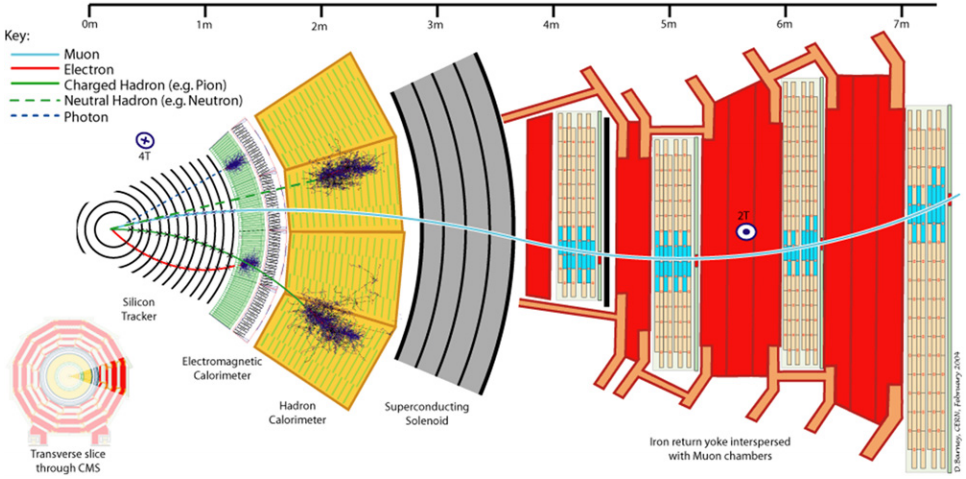
\includegraphics[width=\linewidth]{CMS_detector.png}
    \caption{A sliced view of the CMS detector, courtesy of \cite{ATLASandCMSDetector}. From left to right is the silicon track to trace the motion of the charged particles heading toward the subsequent layers of the ECALs and HCALs. The calorimeters are surrounded by the 4T superconducting solenoid that keeps the beam in a straight line. Finally, subsequent layers of muon chambers to detect the escaping muons surrounds the solenoid.}
    \label{fig:detector}
\end{figure}

\begin{itemize}
  \item \textbf{ECAL}: \par
  The ECALs measure electromagnetic showers that begin with highly energetic electrons and photons. The electrons entering the ECALs produce energetic photons in a process known as Bremsstrahlung, which then further produces a $e^{-}e^{+}$ pair. This process is repeated in the form of an electromagnetic shower until there is not enough energy remaining in the photons or electrons. The electrons and photons interact with atoms in the ECAL through ionisation and scintillation \cite{thomson2013modern}. The CMS detector uses lead-tungstate ($\text{PbWO}_4$) crystals due to its high density and short radiation length. The compact size allows the showers to be contained in a confined region \cite{chatrchyan2008cms}. 
  
  \item \textbf{HCAL}: \par
  The HCALs measure hadronic jets that originate from quarks produced in the collision, and the contribution of missing energy resulting from undetectable particles such as neutrinos and neutral long-lived hadrons. The nuclear interaction between the hadrons and atoms that form the HCAL layers prompt decays of these hadronic jets through ionisation, nuclear interactions, and strong interactions. These interactions form a cascade of interactions as showers, prompted by the alternating-layer structure of the HCAL \cite{thomson2013modern}. The CMS has focused on an alternating-layer structure with brass absorbers to prompt particle interactions, and plastic fluorescent scintillators to emit blue-violet light for detection \cite{chatrchyan2008cms}. 
\end{itemize}

It is possible to identify jets originating from $b$-quarks using a process known as \textit{b-tagging}. The relatively long lifetime of the $b$-quarks means the decays occur at a slight distance away from the collision point (primary vertex), producing a secondary vertex. At the secondary vertex, the $b$-jets form high-mass $B$ hadrons that can decay to highly energetic particles including semi-leptonic products. The tagging of $b$-jets exploit the long lifetime and resolving the secondary vertex, with the track information used to identify particles originating from $B$ hadrons \cite{collaboration_2013}. The identification of $b$-jets less efficient compared to identifying isolated leptons and remains a challenge to improve efficiency. 

%-------------------------------------------------------------------------%
\section{Kinematic variables in collider experiments}
The properties of the measured particles are recorded in the LHC data, with many such properties translated into the transverse plane of the beam axis. This is due to the boosting of many highly energetic particles along the beam axis, which makes it difficult to measure components such as their energy or momentum. Considering the beam direction to be the z-direction the transverse plane would be the $(x,y)$-plane, with the geometry of this depicted in Figure \ref{fig:beam}. \\

\begin{figure}[htbp]
    \centering
    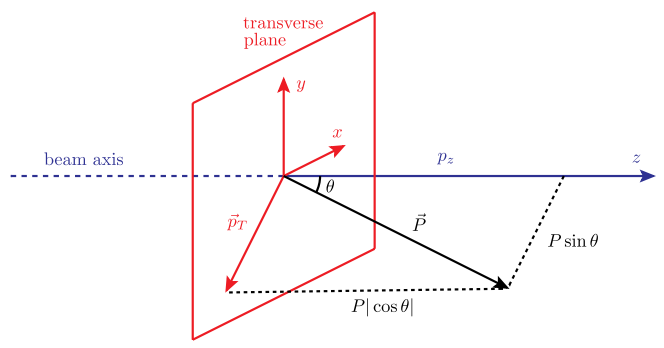
\includegraphics[width=12cm, height= 6cm]{beam.png}
    \caption{The geometry of a collider experiment, with the beam axis considered as the z-direction and the transverse plane as the $(x,y)$-plane \cite{barr2011guide}. The pseudorapidity in Equation (\ref{eq:eta}) measures the polar angle and the azimuthal component $\phi$ is in the $(x,y)$-plane covering $-\pi \leq \phi \leq \pi$. }
    \label{fig:beam}
\end{figure}

One measure in the transverse plane is the transverse momentum, $p_T$, given by, 
\begin{equation}
    p_T = \abs{\overrightarrow{p_T}} = \abs{\sqrt{\overrightarrow{p_x}^2 + \overrightarrow{p_y}^2}}
    \label{eq:pt}
\end{equation}
where $p_x$ and $p_y$ are the momentum of particles in the $x$- and $y$-direction, respectively. It is possible to obtain certain quantities with $p_T$ such as the \textit{missing transverse energy} denoted as $\cancel{\it{E}}_{T}$, and the \textit{scalar transverse energy}\footnote{Otherwise known as the transverse hadronic energy sum.} denoted as $H_T$, given in Equation (\ref{eq:MET}) and Equation (\ref{eq:HT}), respectively. We will refer to the missing transverse energy as missing energy or MET, and the scalar transverse energy as scalar energy or HT from hereon. The missing energy is found by summing over the missing momentum from the detected particles as a consequence of energy and momentum conservation, and the scalar energy is given by the magnitude of the total momentum deposited by hadronic jets. \\
\begin{equation}
    \cancel{\it{E}}_{T} = \abs{\overrightarrow{\cancel{\it{E}}_{T}}} = \abs{- \sum_i \overrightarrow{p_T}(i)}
    \label{eq:MET}
\end{equation}
\begin{equation}
    H_T = \sum_i \abs{p_T(i)} 
    \label{eq:HT}
\end{equation}

In SM decays, leptonic final states of the top quarks produce neutrinos that freely pass through the detector, resulting in some $\cancel{\it{E}}_{T}$. Many MSSM events are predicted to have a large excess of $\cancel{\it{E}}_{T}$, more than the SM processes, due to a larger number of undetectable particles from the lightest neutralinos.  \\ 

%-------------------------------------------------------------------------%
\section{Simulations of a collider}
\label{sec:Sims}
The data collected in collider experiments do not contain labels associated with the physical processes measured. By simulating the process of interest closely following known theory and calculations, the existence, or lack of, the process of interest in the raw data can be identified by statistical techniques. There are typically three stages of simulation: the production/generation of the events through $pp$ collisions, the hadronisation of quarks leading to parton showers, and finally, the detection of electrons, muons, photons and jets as listed in Section \ref{sec:Detector}. \\

The generator level simulation of choice was MadGraph5\_aMC@NLO \cite{alwall2014automated} (MadGraph or MG5) due to its simplicity and fully-automated chain of simulations leading to the detector output. MadGraph calculates the cross-sections of the events of interest at leading-order (LO) by default\footnote{There is the capability for Next-to-leading-order (NLO) calculations as well, but we stick to the default LO calculations.}. However, the events do not mimic an output of the detector exactly and to achieve the complete simulation, these events must be processed further into what a real detector may observe. The intermediate steps such as hadronization of the quarks and their showers are governed by PYTHIA8.2 \cite{sjostrand2015introduction}, integrated into MadGraph, through Monte Carlo simulations. The output created by PYTHIA (HepMC files) may be fed directly into a detector level simulation of choice. \\

Delphes3 \cite{de2014delphes} is the detector level simulation chosen for this project due to its MG5 build-in feature, making the simulation process a single chain of operation. The CMS detector card was chosen to input parameters identical to selection criterion from CMS experiments \cite{cms2019search, cms2016searches, cms2017search}, shown in Table \ref{tab:efficiencies}. Jets are found through the FastJet finder \cite{cacciari2012fastjet} applying the anti-$k_t$ algorithm \cite{cacciari2008anti}. The output is a smeared calculation to the particle properties, in which isolated leptons, photons, jets, and $\cancel{\it{E}}_{T}$ are some of the main components reconstructed. Other information such as the track and vertices are also calculated. Muons are detected with an efficiency of 95\% while the electrons are detected with an efficiency of 85\%. Both leptons with a minimum $p_T$ of 20 GeV are considered to be isolated when it remains within a cone radius of $\Delta R <0.2$ and satisfies $I(l)<0.1$, given by Equation (\ref{eq:iso}) \cite{de2014delphes}. We require isolated leptons as they provide well-studied signatures from the SM that can be associated with new signatures from the weak interaction at high energies \cite{diaconu2004isolated}. The jets are identified when they have a minimum $p_T$ of 30GeV within a cone radius of $\Delta R <0.4$, with those originating from $b$-quarks are tagged with a lower efficiency of 60\%. \\

\begin{table}[htbp]
    \centering
    \begin{tabular}{c|c}
    \toprule
    Particle Type & Input parameters for the detector simulation \\
    \midrule
    \rowcolor{gray!6} Electrons & $\abs{\eta} < 1.442$, $p_T > 20\text{ GeV}$ @ $85\%$, $\Delta R <0.2$, $I(l) <0.1$\\
    Muons & $\abs{\eta} < 2.4$, $p_T > 20\text{ GeV}$ @ $95\%$, $\Delta R < 0.2$, $I(l) <0.1$\\
    \rowcolor{gray!6} Jets & $p_T>30$ GeV, $\Delta R = 0.4$\\
    b-tagging & $60\%$ \\
    \bottomrule
    \end{tabular}
    \caption{Chosen efficiencies for our detector simulation. The isolated electrons are 10\% less efficiently identified than isolated muons, also covering a narrower $\eta$ range. The isolation variable defined by Equation (\ref{eq:iso}) determines which charged electrons and muons from the detected particles are isolated, given a minimum $p_T$ of 20 GeV. The jets have a cone size of $\Delta R = 0.4$ travelling with $p_T>30$ GeV, where 60\% of those originating from $b$-quarks are tagged correctly.} 
    \label{tab:efficiencies}    
\end{table}

\begin{equation}
    \left. I(l) = \sum\limits_{i\ne l}^{R<\Delta R} p_T(i) \middle/ p_T(l) \right. \\
    \label{eq:iso}
\end{equation}


For this project, we stick to the properties listed in Table \ref{tab:variables}, including $H_T$, where leptons up to second-order and jets up to fourth order are selected. In addition, each of the jets will have an associated entry as to whether it is b-tagged or not. This information will be important to our analysis in the upcoming section. \\ 


\begin{table}[htbp]
    \centering
    \begin{tabular}{c|c|c|c} 
    \toprule
     & $\cancel{\it{E}}_{T}$ & $l^{\pm}_{i=1,2}$ & $j_{i=1,2,3,4}$ \\
    \midrule
    \rowcolor{gray!6} Energy & $\abs{\cancel{\it{E}}_{T}}$ & $ p_{T_l} $ & $ p_{T_j} $ \\
    $\eta$ & $\eta_{\cancel{\it{E}}_{T}}$ & $ \eta_l $ & $ \eta_j $ \\
    \rowcolor{gray!6} $\phi$ & $\phi_{\cancel{\it{E}}_{T}}$ & $ \phi_l $ & $ \phi_j $ \\
     %&  & $  $ & $  $\\
    \bottomrule
    \end{tabular}
    \caption{The variables extracted are the energy, $\phi$ and $\eta$ components of the MET, two charged leptons (one of which is a veto), and the four jets with a minimum of one $b$-tag were chosen.} 
    \label{tab:variables}
\end{table}

%-------------------------------------------------------------------------%
\section{Cut-based searches}
\label{sec:cut}
The cut-based analysis is an intuitive approach to the analysis of data from collider experiments, in which events are accepted or rejected based on physically motivated criteria. The objective of this method remains the same: to discriminate signal against background events and increase the sensitivity of the signal. An example diagram is shown in Figure \ref{fig:cut_flow}, where varying criterion (Recall Section \ref{sec:Detector}) such as $x>a$, $y>c$ and a multivariate variable $f(x,y)$, a combination of variables $x$ and $y$, accepts and rejects events. It results in the minimum number of background events remaining while maintaining a significant portion of signal events.  \\

\begin{figure}[htbp]
    \centering
    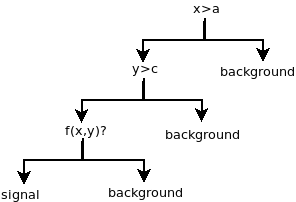
\includegraphics[width=0.5\linewidth]{cut_flow.png}
    \caption{A diagram depicting cut-flow analysis. For some criterion $x>a$, $y>c$ and a multivariate variable $f(x,y)$, the cuts accept events that satisfy such criteria, discarding events as background otherwise.}
    \label{fig:cut_flow}
\end{figure}

The benefit of cut-based searches is that these cuts are physically well-motivated and easy to keep track of. However, this may also be negative in certain scenarios where the physical properties of the particle in question are not as evident or well known. Searches for the process $\Tilde{t}\Tilde{t}^*  \rightarrow t\bar{t}\Tilde{\chi}_1^0\Tilde{\chi}_1^0$, but not limited to, have made use of a range of variables including $\cancel{\it{E}}_{T}$, the transverse mass $M_T$, the azimuthal difference between $\cancel{\it{E}}_{T}$ and a given jet, $\Delta \phi (\cancel{\it{E}}_{T}, \text{jet})$, and the number of specific particles within the data \cite{kraml2016scalar, chatrchyan2013search}. The cut-based analysis complements machine learning algorithms as a form of pre-selection technique that reduces background and signal events to similar signatures.